\section{引言}
\label{sec:intro}

在 sRGB 显示值中做线性插值，建模的是光的加色混合，而非颜料的减色混合。对类颜料介质，三处差异总是可见。第一，蓝色与黄色颜料得到绿色，而蓝色与黄色光得到去饱和的中性色。第二，互补颜料得到浑浊的棕、橄榄与暗紫，而互补光趋向灰色。第三，深色颜料加白后仍保持色度并发生色相偏移，而 RGB 插值会朝灰白去饱和。这些行为都不是显示值的线性组合能给出的；\cref{fig:overview} 以深蓝颜料分别与亮黄颜料、与白色混合为例说明这一点。

颜料混色的物理参考是 Kubelka--Munk（K--M）双流模型。对不透明层，反射率为 $\Rinf(\kappa)=1+\kappa-\sqrt{\kappa^{2}+2\kappa}$，其中 $\kappa=K/S$；Duncan 指出混合物的吸收与散射系数按浓度线性叠加 \cite{kubelka1931,duncan1940}。结合光源与 CIE 标准观察者，该模型能够复现颜料层的大部分定性与定量行为 \cite{haase1992,wyszecki2000}。然而它在交互软件中的使用受限于接口而非前向模型：K--M 需要逐颜料光谱，而任意 RGB 颜色并不提供这些数据；混合两个 RGB 输入还需要数值反解模型。在我们的测量中，RGB 到颜料浓度的反解使一次光谱混色操作的成本约为本文解析模型的 $10^{5}$ 倍（\cref{sec:runtime}）。另一个限制是色域：某些 RGB 颜色无法由任何可用颜料混合得到 \cite{pointer1980}。

Mixbox \cite{sochorova2021} 通过从实测颜料光谱学习每个 RGB 颜色的七维潜表示、对潜向量线性插值、再用预计算的 $256^{3}$ 表解码回 RGB，使基于 K--M 的混色变得实用。该模型能紧密复现颜料行为，本文以它作为参考。其映射是训练得到且基于查找表的，参考实现又以非商业许可分发；这些性质促使我们寻求解析替代，而不是取代参考所依赖的实测数据。

本文描述颜料基混色（PBM），一个直接作用于 sRGB 显示值的解析模型。PBM 保留 K--M/Duncan 混色的结构要素——浓度加权的吸收与散射、跨通道混合矩阵、互吸收修正——并增加一个修复层，用以补偿 K--M 在显示值空间中的唯一结构性缺陷：近白颜色的散射项主导混合物分母，把深色颜料的吸收冲淡（\cref{sec:defect}）。修复层由三层连续混合的机制组成：针对深色加白的逐通道幂律目标、针对互补色对的加性谐波修正，以及使整体模型交换对称的软角色分配。

我们明确模型的适用范围。PBM 是\emph{参考校准}的：其常数由反解并拟合 Mixbox~2.0 的输出得到，而该参考的潜空间训练自实测颜料光谱。因此模型是对参考的近似，它与真实颜料的关系被参考自身与真实颜料的关系所界定。本文使用\emph{物理启发}一词，仅描述与 K--M/Duncan 混色的结构对应；没有任何拟合常数来自颜料物理，评估也不包含实物颜料样品的测量。

\paragraph{设计目标.}
我们以三个对交互软件有意义的目标评估模型：
\begin{enumerate}[label=R\arabic*.,leftmargin=2.2em]
\item 在 sRGB 显示值上运算，RGB 输入、RGB 输出，不需要光谱数据或额外的逐像素通道；
\item 接受全部 RGB 颜色，在 $\alpha=0$ 与 $\alpha=1$ 处精确返回输入，并随输入连续变化；
\item 完全解析：无查找表、无训练数据、无迭代，以便能被独立重新实现。
\end{enumerate}

\paragraph{贡献.}
\begin{itemize}
\item 一个作用于 sRGB 显示值空间的解析两阶段混色模型：K--M/Duncan 结构的核心 + 连续混合的修复层（\cref{sec:model}）。
\item 无三角函数的谐波修正：在十七个通道比值特征上的线性模型，使整个模型只使用算术、幂与平方根（\cref{sec:repair}）。
\item 可复现的参数估计流程：谐波系数由最小二乘闭式求解，其余标量由坐标下降得到（\cref{sec:estimation}）。
\item 消融与门控敏感性研究，以及端点恒等、邻域连续性、交换对称与运行时间的测量（\cref{sec:evaluation}）。
\item 相对 Mixbox~2.0 的评估，含显式的样本内/留出划分与 bootstrap 置信区间，并以独立合成光谱世界交叉验证（\cref{sec:results,sec:synthetic}）。
\item 对评估不能确立之事的明确说明（\cref{sec:threats,sec:limitations}）。
\end{itemize}

\Cref{tab:positioning} 概括定位。后文依次回顾背景（\cref{sec:background}）、形式化模型（\cref{sec:model}）、描述参数估计（\cref{sec:estimation}）、报告评估（\cref{sec:evaluation}）并讨论局限（\cref{sec:limitations}）。

\begin{table}[t]
\centering
\small
\caption{相对设计目标 R1--R3 的定位，以及与 Mixbox~2.0 的实测精度（平均 $\Delta E_{00}$；样本内 T5 与留出 T3，\cref{sec:results}）。}
\label{tab:positioning}
\begin{tabular}{lccccc}
\toprule
模型 & R1 & R2 & R3 & T5 均值 & 留出 T3 均值 \\
\midrule
PBM（本文） & \checkmark & \checkmark & \checkmark & 2.26 & 2.72--2.85 \\
Mixbox 2.0 \cite{sochorova2021} & \checkmark & \checkmark & $\times$（训练 $256^{3}$ 查找表） & 参考 & 参考 \\
RGB 插值 & \checkmark & \checkmark & \checkmark & 8.13 & 3.27--3.46 \\
原始 K--M 叠加 & \checkmark & \checkmark & \checkmark & 10.30 & 3.92--4.01 \\
\bottomrule
\end{tabular}
\end{table}

\begin{figure}[t]
\centering
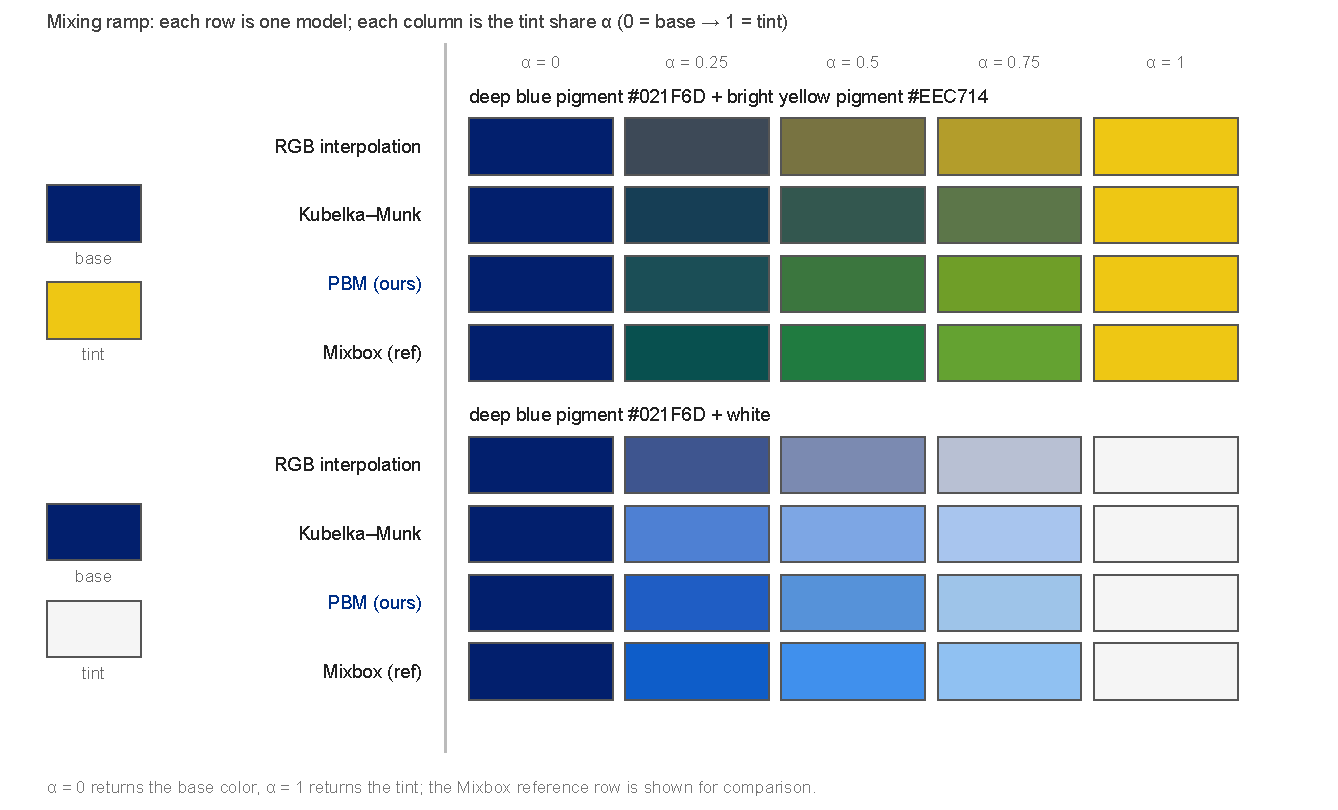
\includegraphics[width=\linewidth]{fig1-mixing.pdf}
\caption{RGB 插值、光谱 K--M、PBM 与 Mixbox 参考的混色行为。上：深蓝颜料与亮黄颜料混合。下：同一深蓝与白混合。每行一个模型；每列为染色占比 $\alpha$（$\alpha=0$ 返回基色，$\alpha=1$ 返回染色）。K--M 行为 \cref{sec:synthetic} 的合成光谱真值：合成颜料光谱经两常数 Duncan 叠加，输入为纯颜料的渲染色。PBM 遵循同样的定性族（黄 $\times$ 蓝 $\rightarrow$ 绿；深 $+$ 白保持色度）。}
\label{fig:overview}
\end{figure}
